%
% ---------------------------------------------------
%
% Proyecto de Final de Carrera:
% Author: Alejandro Hernández Padrón <alu0100703511@ull.edu.es>
% Capítulo: Objetivos 
% Fichero: Cap1_Goals.tex
%
% ----------------------------------------------------
%


\chapter{Beacons en entornos universitarios} \label{chap:BeaconsEntornosUniversitarios}  


En este capítulo realizaremos un análisis de los posibles casos de uso de la tecnología beacon en el ámbito universitario.

 
\section{Aplicaciones móviles en entornos universitarios}


Actualmente las posibilidades de las aplicaciones móviles para entornos universitarios se presentan amplias.  Cada universidad intenta tener su propia aplicación siguiendo un patrón similar, puesto que todas parten de necesidades similares. Realizando una investigación general de las aplicaciones disponibles en el mercado observamos que estas aplicaciones se centran en ofrecer servicios propios (servicio de correo, Moodle, chat entre usuarios, etc.), mantener al alumnado informado y agilizarle los trámites mayoritariamente. 

En un principio, estas aplicaciones se enfocaban a atraer estudiantes, centrándose en la calidad de la universidad y mostrando las posibilidades que ofrecían. Sin embargo, con el paso de los años y el desarrollo creciente de las aplicaciones móviles, se muestra un cambio en esta estrategia. Ahora las aplicaciones tienen una doble función y no sólo buscan el acceso de nuevos estudiantes, sino que también intentan mejorar la experiencia del alumnado ya matriculado y acercar a los nuevos a la experiencia de la universidad. 
Algunos ejemplos posibles los encontramos en el marketplace de Google \cite{URL::galileo, URL::valladolid, URL::oviedo}


Uno de los hechos que podemos observar es que las universidades están intentando obtener una solución rápida para desarrollar su app. Una de estas soluciones es la creación de plantillas web optimizadas de su sitio web, lo que podemos considerar una opción rápida con un coste bajo.


Hoy en día casi todos los estudiantes tienen acceso a un dispositivo móvil y cuentan con una tarifa de internet. En un futuro próximo con la aparición de estos dispositivos ya nos surge la pregunta ¿Serán capaces estos dispositivos de transformar la educación? y en caso afirmativo ¿De qué manera? 

\section {Posibles casos de uso de la tecnología beacon en entornos universitarios}

Como se mencionaba antes, una de las posibilidades que se presentan para explotar esta tecnología se encuentra en las instituciones de enseñanza, las cuales podrían utilizar los beacons para facilitar a su alumnado, profesorado y demás personal involucrado  una serie de servicios de gran utilidad.


Sin embargo, para utilizar esta tecnología es necesario cumplir una serie de condiciones:

\begin{itemize}
\item Tener instalada la aplicación en su dispositivo móvil.
\item Tener activado el protocolo Bluetooth.
\item La aplicación ha de estar activa.
\item Los beacons han de estar desplegados y configurados correctamente en lugares clave donde el rango sea óptimo.
\end{itemize}

En el caso de dispositivos Apple no es necesario tener activado el Bluetooth ya que el SO se encarga de captar las señales BLE. Tampoco es necesario que la app esté despierta ya que nuevamente el SO se encarga de despertar a la aplicación involucrada. Sin embargo Apple no ha desarrollado un IBeacon físico aún, aunque en un futuro, se espera que sus dispositivos móviles puedan funcionar como un beacon bidireccional. Cabe destacar que existen librerías que se encargan de realizar estas mismas funcionalidades para mantener el móvil despierto a la escucha de posibles beacon para otros sistemas operativos, pero a diferencia de Apple esta funcionalidad no está integrada directamente en el SO por lo que no presenta el mismo nivel de control.


Asimismo, podemos afirmar que prácticamente la mayoría de las universidades cuentan con una disposición amplia en lo que se refiere a servicios y despliegue de medios. Como ejemplo, podemos tomar la Universidad de la Laguna, la cual cuenta con una red WiFi con un rango de cobertura casi completo en sus instalaciones y una amplia carta de servicios disponibles para sus alumnos. Además cuenta con una serie de beacons, que podrían ser instalados fácilmente en lugares estratégicos. 

Partiendo de esta base, procederemos a explorar posibles casos de uso para los beacons tomando el contexto universitario y del alumnado como referente:

\subsection{Guía a través del campus de la universidad}

Este caso de uso cubre la funcionalidad principal de un beacon. El posicionamiento y guía tanto en exteriores como en interiores. 

Como interesados podríamos destacar: 

\begin{itemize}
\item Personal invitado a jornadas o eventos en instalaciones de la universidad.
\item Alumnado de intercambio en programas internacionales.
\item Estudiantes de nuevo acceso.
\item Personas con discapacidad.
\end{itemize}

\begin{figure}[h]
	\centering
	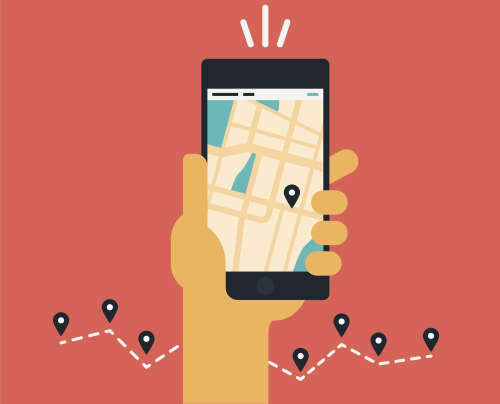
\includegraphics[width=0.6\linewidth]{locationMobileBeacon}
	\caption{Servicios de localización a través de la Universidad}
	\label{fig:beaconLocation}
\end{figure}

El funcionamiento sería el siguiente: el usuario transita por las inmediaciones del campus universitario. El usuario accede al sistema de navegación dentro de la aplicación, la cual le muestra entonces su ubicación como un punto de color sobre el mapa del campus. Este mapa tiene marcados puntos de interés que contienen información de diferente tipo dependiendo del punto marcado: nombre, historia, página web, teléfono de contacto, trámites asociados... son algunos de los datos que podría mostrar. El mapa se va actualizando dependiendo de la posición del usuario permitiendo volver a la vista más alejada en cualquier momento para una visualización más general.


\subsection{Descarga automática de material} \label{sec:descargaautomatica}

Este caso de uso resultaría muy útil para personal lectivo y para estudiantes, los cuales accederían de manera más sencilla al material disponible. También sería aplicable para ponentes de charlas quienes no tendrían que alojar sus apuntes en alguna plataforma externa o llevarlos consigo en  un almacenamiento externo para compartirlo al finalizar la actividad.

El funcionamiento sería el siguiente: el profesor/a o ponente lleva consigo un beacon y sus estudiantes u oyentes tienen instalados en sus dispositivos la aplicación. El profesor es capaz de introducir en su aplicación con el perfil de profesor (el ponente con su correspondiente perfil), indicaciones del material a utilizar en el evento. El profesor/a carga consigo el pequeño dispositivo e indica al alumnado que conecten el Bluetooth y abran la aplicación. Al entrar en el rango, la app pedirá permiso al alumno para descargarse el contenido indicado por el profesor. Si el alumno acepta, la aplicación pasaría a abrir  el contenido indicado por la página correspondiente.


\subsection{Acceso al parking y recuento de número de plazas disponibles}


Este caso de uso proporcionaría información muy útil a los usuarios del parking de la universidad, informando del número coches estacionados en el parking y de las plazas restantes a ocupar en tiempo real.

El funcionamiento sería el siguiente: el personal de la ULL tendría la aplicación en su móvil; al acercarse a la barrera del parking, el usuario activaría el Bluetooth de su móvil. La app registraría un nuevo punto entrando en el rango de acción del parking. La aplicación comprobaría conectando con un servidor institucional que el usuario está autorizado a entrar en el parking y procedería a abrir la puerta del parking dejando entrar al vehículo. Cuando el vehículo saliese del rango del beacon por el rango interior, la aplicación registraría entonces un nuevo acceso al parking y contabilizaría otro vehículo dentro de parking. Al salir del parking el proceso sería el mismo, por lo tanto la aplicación sería capaz de informar al usuario de las plazas ocupadas en tiempo real.


\subsection{Gestión de eventos e información, entrada automática}

El funcionamiento sería el siguiente: el alumnado transita los interiores de la Universidad de camino a sus clases. Los beacons están desplegados en las inmediaciones de lugares de interés, tipo aulario, paraninfo, clases que se utilicen a modo de salas de reuniones o seminarios. Al pasar por las inmediaciones de estos lugares de interés, la aplicación sería capaz de proporcionar al usuario información de diversa índole: ponentes, tema de la charla, acceso, teléfono de contacto u otra información similar.  Al mismo tiempo, la aplicación también cuenta con un tablón donde se muestran posibles eventos futuros. Estos eventos pueden ser muy variados y corresponder a diferentes tipos de actividades. Al mismo tiempo se podría confirmar la entrada al evento en el caso de haberla, mediante un código de acceso identificativo generado al realizar la inscripción en el evento.

\begin{figure}[H]
	\centering
	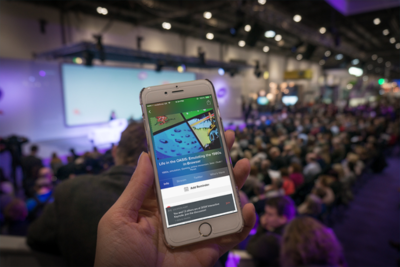
\includegraphics[width=0.6\linewidth]{BeaconEvent}
	\label{fig:eventBeacon}
	\caption{La aplicación presenta información al usuario sobre el evento que está teniendo lugar.}
\end{figure}

\subsection{Despacho del profesorado e información}

El funcionamiento podría ser abarcado de dos maneras. Por un lado, podría utilizarse para proveer al alumnado de información acerca del grupo de despachos, aclarando que profesorado tiene el despacho en la zona, horario de tutorías, correo electrónico de contacto, horario de corrección de exámenes, etc. De esta manera el alumnado al acercarse a la zona sería capaz de acceder a información de todo el profesorado, o si buscase a alguno en particular, la aplicación le daría la opción de elegir su nombre de una lista y simplemente comprobar si tiene su despacho en esa zona. 

Por otro lado, este caso de uso podría ampliarse para proporcionar una información adicional, comprobando si el profesorado está en la zona en ese momento y se encuentra disponible. El profesor tendrá un perfil de la aplicación con un código identificativo que le distingue de los demás profesores. Estos datos se guardarían en un servicio externo, y la app sería la encargada acceder a este servicio consultando las entradas y salidas del profesorado. De esta manera el alumnado sería capaz de saber cuando el profesor se encuentra disponible en las cercanías mediante la aplicación. En cuanto al estado de disponibilidad, sería un dato que actualizaría el profesor desde su perfil en la aplicación. 

\subsection{Información y descuentos para usuarios de la app}

Este caso de uso no solo dependería de la universidad, sino de establecimientos comerciales interesados. La idea sería la siguiente: la universidad en colaboración con un establecimiento comercial le entrega un beacon. La aplicación contaría con un perfil para el dueño del establecimiento, donde sería capaz de introducir información que desea que se muestre al usuario al pasar cerca de su establecimiento, mensajes de información, descuentos u ofertas especiales por ejemplo. 

El usuario al pasar por las inmediaciones del establecimiento recibe en su aplicación una notificación del establecimiento con la información introducida por el dueño anteriormente. Al aceptar la notificación, el usuario podría ser redirigido a la página web del establecimiento para ver las ofertas. En cualquier caso el establecimiento ha conseguido captar la atención de un posible cliente, y el usuario se beneficiaría de ofertas y descuentos. 

\subsection{Control de asistencia}

Este caso de uso puede ir ligado al de descarga automática de material (véase epígrafe \ref{sec:descargaautomatica}), el funcionamiento sería el siguiente: el alumno conectaría el Bluetooth de su móvil al iniciar la clase. En ese momento la aplicación detectaría los dispositivos y permitiría al usuario registrar su asistencia a la clase en el horario lectivo. El profesorado sería capaz en todo momento, desde el perfil del profesor, de consultar la asistencia de los alumnos. Si lo unimos a la descarga automática de material, proporcionaría comodidad tanto al alumnado como al profesorado. Sin embargo, un impedimento podría ser el rango del beacon o la necesidad de activar el Bluetooth ya que, si el alumno no tiene batería en el móvil, habría que recurrir a un método secundario. 

\subsection{Control de acceso a instalaciones}

El control de acceso a las aulas y edificios puede ser un tema abordable mediante el uso de estos dispositivos. Los lectores de tarjetas pasarían a ser algo innecesario. El alumno simplemente tendría que activar el Bluetooth cerca del punto de entrada, se comprobaría su identidad y se procedería a darle a acceso o a informarle de su falta de permiso. Los permisos para acceder a estos puntos podrían quedar almacenados en alguna plataforma donde se puedan visualizar.

\subsection{Biblioteca informativa}

Otro posible uso de la tecnología beacon tiene que ver con las bibliotecas o lugares de almacenamiento de material. El estudiante se acercaría a la biblioteca buscando un libro específico. Partimos de que en la app estaría registrada la localización de los libros disponibles en los estantes. De esta manera la aplicación indicaría al alumno o alumna la posición del libro que busca. Para lugares amplios donde hay gran cantidad de material (véase la Figura \ref{fig:bibliotecaUSAL}), incluso podría guiar al usuario por las instalaciones hasta llegar a su objetivo, informarle del número de ejemplares disponibles o de la fecha prevista de entrada de algún título.

\begin{figure}[H]
	\centering
	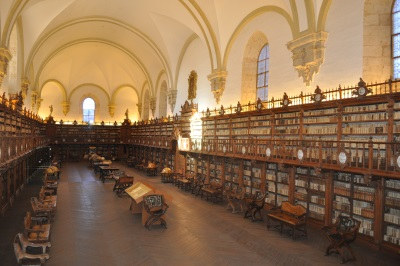
\includegraphics[width=0.6\linewidth]{BibliotecaSalamanca}
	\caption{La biblioteca de la Universidad de Salamanca contiene más de 1.000.000 de ejemplares lo que puede dificultar la localización de algunos títulos.}
	\label{fig:bibliotecaUSAL}
\end{figure}

\subsection{Actividades interactivas por el campus, jornadas de acogida u otros eventos}

En un ámbito más recreativo, se podría tener en cuenta el uso de los beacons para organizar juegos o actividades de ocio para el alumnado. Por ejemplo, rutas a través del campus con adivinanzas o puzzles relacionados con diferentes temáticas, lo que fomentaría el trabajo en equipo. Al mismo tiempo se podría aplicar algún tipo de recompensa para los ganadores, descuentos o bonos tramitados por medio de la aplicación. Estos eventos dependerían de los organizadores y el alumnado tendría que registrarse con su identificador. 

\subsection{Localización de transporte público, horarios e \\información de la parada}

Uno de los transportes más utilizados por el alumnado de la universidad es el autobús. Este medio de transporte puede llegar a ser el día a día de muchos de los estudiantes que no cuentan con vehículo propio o que simplemente prefieren utilizar este medio de transporte. 

Este caso de uso contempla lo siguiente: el estudiante llega a una parada de autobús y utilizando su dispositivo móvil, consulta los autobuses que van a pasar por la parada. La aplicación le permite obtener información de los diferentes autobuses, el itinerario y el tiempo restante para que llegue a la parada.  Asimismo enlazaría con la web de la compañía de transporte para información adicional sobre líneas e itinerarios.
